\documentclass[english]{lni}

\usepackage{url}
\usepackage{hyperref}
\usepackage[utf8]{inputenc}
\usepackage{nameref}
\usepackage{graphicx}
\usepackage{tabularx}
\usepackage{adjustbox}

%nothing works related to colored tables
%\PassOptionsToPackage[table]{xcolor}
%\usepackage[table]{xcolor}  % https://tex.stackexchange.com/questions/83101/option-clash-for-package-xcolor
%\usepackage{xcolor}
\usepackage{array}   % table col width in tabular {}
\usepackage[normalem]{ulem}
\useunder{\uline}{\ul}{}


%%% overleaf doku:   https://de.overleaf.com/learn/latex/Bibliography_management_in_LaTeX
\usepackage[
backend=biber,
style=alphabetic,
sorting=ynt
]{biblatex}
\addbibresource{mybibfile.bib}
% \addbibresource{mybibfile}    % lni.dtx  Z.615ff

\begin{document}
%\title[Cloud Computing: SciTube] {A scientific Video-on-Demand-Solution powered by Microsoft Azure}
\title{Cloud Computing: SciTube}
\subtitle{A scientific Video-on-Demand-Solution powered by Microsoft Azure}
\author[Markus Herche \and Benjamin Hildebrandt]
{Markus Herche\footnote{Hochschule Fulda, Dept. of Computer Science, Leipziger Straße 123, 36037 Fulda,
Germany \email{markus.j.herche@cs.hs-fulda.de}} \and
Benjamin Hildebrandt\footnote{Hochschule Fulda, Dept. of Computer Science, Leipziger Straße 123, 36037 Fulda,
Germany
\email{benjamin.hildebrandt@cs.hs-fulda.de}}}

\booktitle{Cloud Computing} % Name of book title
\editor{Markus Herche \& Benjamin Hildebrandt} % Names of Editors
\booktitle{SciTube} % Name of book title
\year{2018-2019}


\maketitle

\begin{abstract}
    The saying goes that a picture says more than a thousand words. This should apply to scientific papers as well,
    because why describe e.g. the deformation of a curve, when that can just be shown in a quick video. The following 
    paper outlines a basic cloud-based video-on-demand-solution with a pay-per-view-model. 
\end{abstract}

Note: This project made possible through the Microsoft Azure Academic Program.

% Verlage wollen Geld, Autoren wollen Geld, wir wollen Geld für die Serverkosten.
% Ohne Geld nur Preview, Live-Streaming von Konferenzen und Keynotes, billiger als Ticket + Reise.
% Springer Article 6 Seiten: 40 Euro

Although it is possible to find scientific content and thorough explanations
of complex materia on established platforms like YouTube, it can be
hard to find among other non-science related stuff. Discussion of topics 
is also limited as the comment sections tend to either be full of unanswered questions
or just typical internet madness. By creating a platform for professionals,
that might hopefully change.\\

Monetization is also an important factor as established publishers of journals
seem content to charge around 40 euros for an article, as in: a six-page-excerpt of a journal.
This is a strong indication that enriched content can also be charged for.\\
On Project \textit{SciTube}, Users can create and publish Videos and recorded 
talks and cut out a preview for all other
users. This feature coupled with a rating-system should make it easier 
for interested viewers to decide if they should pay for the whole thing.
Creators can also decide to make the video free for everyone, which 
introduces ads to at least try and cover server costs.\\
% wieviel Werbeeinnahmen bekommt man denn so?
A richer discussion through comments could be made possible through a 
community-based moderation-system similar to platforms like StackExchange.
Users can gain reputation for quality content and proven experts
(say, Doctors and Professors) could contact the team and receive extra reputation
upon proof of academic success.

% Ähnlich Stack Overflow etc: Community-Moderation durch ausgewiesene Fachkräfte, die Reputation sammeln können
% (zb: Interessierte Profs und Doktoren melden sich mit Nachweis an, erhalten direkt +100 Reputation in ihrem Fachgebiet)\\


\section{Microsoft Azure Fundamentals}\label{sec:ch2}Microsoft offers both \textit{Infrastructure} and \textit{Platform} as a Service through Microsoft Azure for customers to use and implement Software as a Service. Management functionality itself is provided as SaaS as well (accessible through Webbrowser and REST-API). Applications consist of multiple \glqq building blocks\grqq{} that can be managed individually, but organized together in \textit{resource groups}. These are groups for sorting and encapsulating different services or parts of one service. Every other component have to be in such a \textit{resource group}. 

Managing and Configuring can be done via GUI in any Webbrowser through the Azure portal \footnote{\url{portal.azure.com}} or through \textit{Azure CLI} (Command Line Interface) scripts (similar to Shell- or Batch-scripts). Those can be exported from the GUI for easy reuse, minimizing the risk of missing a checkbox or a specific option. To run such scripts locally, it's necessary to install software \footnote{\url{https://docs.microsoft.com/de-de/cli/azure/install-azure-cli?view=azure-cli-latest}}, which introduces platform-dependency. Parameters for options can be enclosed in high commas on Linux-systems, but must be put in double quotes on Windows.

Azure CLI commands (for the most part) have the following pattern:\\
\texttt{az [resource-type] [action] [--option 'parameters'] [further options]}\\
Upon execution they either terminate with an error message or by printing a JSON received from Azure on success, offering details about the performed action.
% Lästig: manche Bezeichner (zb für Storage Accounts, logischerweise AppService für die Subdomain) müssen in Azure eindeutig sein, manche nur innerhalb der eigenen Ressourcensammlung\cite{azNaming}. erschwert kollaboration und versionierung, wenn skripte sich durch namen unterscheiden 
% Unterschiede zwischen Bash und cmd-Skripten (azcli on Windows vs Linux bzw. WSL) bei parametern: Hochkommata vs Anführungszeichen
% AZCLI-Kommandos beginnen mit az, geben dann (ggf. Ressourcentyp) und die Aktion an. Als Antwort gibt es JSON mit Komplettinfos über die erstellte Instanz

Azure provides many service solutions where one is a Video-on-demand service. This implementation is shown in figure \ref{fig:arch_new} and contains the following cloud components\footnote{\url{https://azure.microsoft.com/en-gb/solutions/architecture/digital-media-video/}}:
\begin{itemize}
    \item \textbf{BlobStorage:} Can store a large amount of unstructured data and can be accessed from anywhere by using http or https. Here the files will be stored.
    \item \textbf{Streaming Endpoint:} Deliveres content directly to a player application or to a content-delivery network (CDN).
    \item \textbf{Azure Encoder:} Creates jobs, which convert media files from one encoding to another.
    \item \textbf{Azure CDN:} Delivers content with a broad global reach.
    \item \textbf{Azure Media Player:} A player application which can be used to directly stream media files from \textit{Streaming Endpoints}.
    \item \textbf{Multi-DRM content protection:} Multi-DRM or AES clear key encryption.
\end{itemize}
\section{Our Implementation}\label{sec:ch3}
%Follows the proposed architecture from Microsoft themselves\cite{azVODArchitecture}, then again, what else would you add for VOD.
%\begin{itemize}
%    \item BlobStorage
%    \item AppService
%    \item Streaming Endpoint
%    \item Azure Media Services: Encoding and DRM
%    \item  .....
%    \item   \textbf{Bild noch rein}
%\end{itemize}
%Using Streaminglocator for adaptive streaming via HLS or Mpeg-DASH. 
A modification of the in section \ref{sec:ch2} proposed architecture was implemented because of cost issues and is shown in figure \ref{fig:arch_new}. To get a fast overview of all uploaded videos and mask the underlaying Azure architecture of the service and its credentials, a Node.JS webserver along a sql database is used as interface between user and service. After the user specified a file, it is uploaded to the webserver where a asset and a corresponding job is created by calling the Azure API. After processing and uploading successfully all information are stored in the database and the file is deleted from the webserver. These information contain a Azure streaming URL. This specific URL is used to stream the video directly from Azure by inserting in a Azure Media Player.
\begin{figure}[ht]
    \centering
    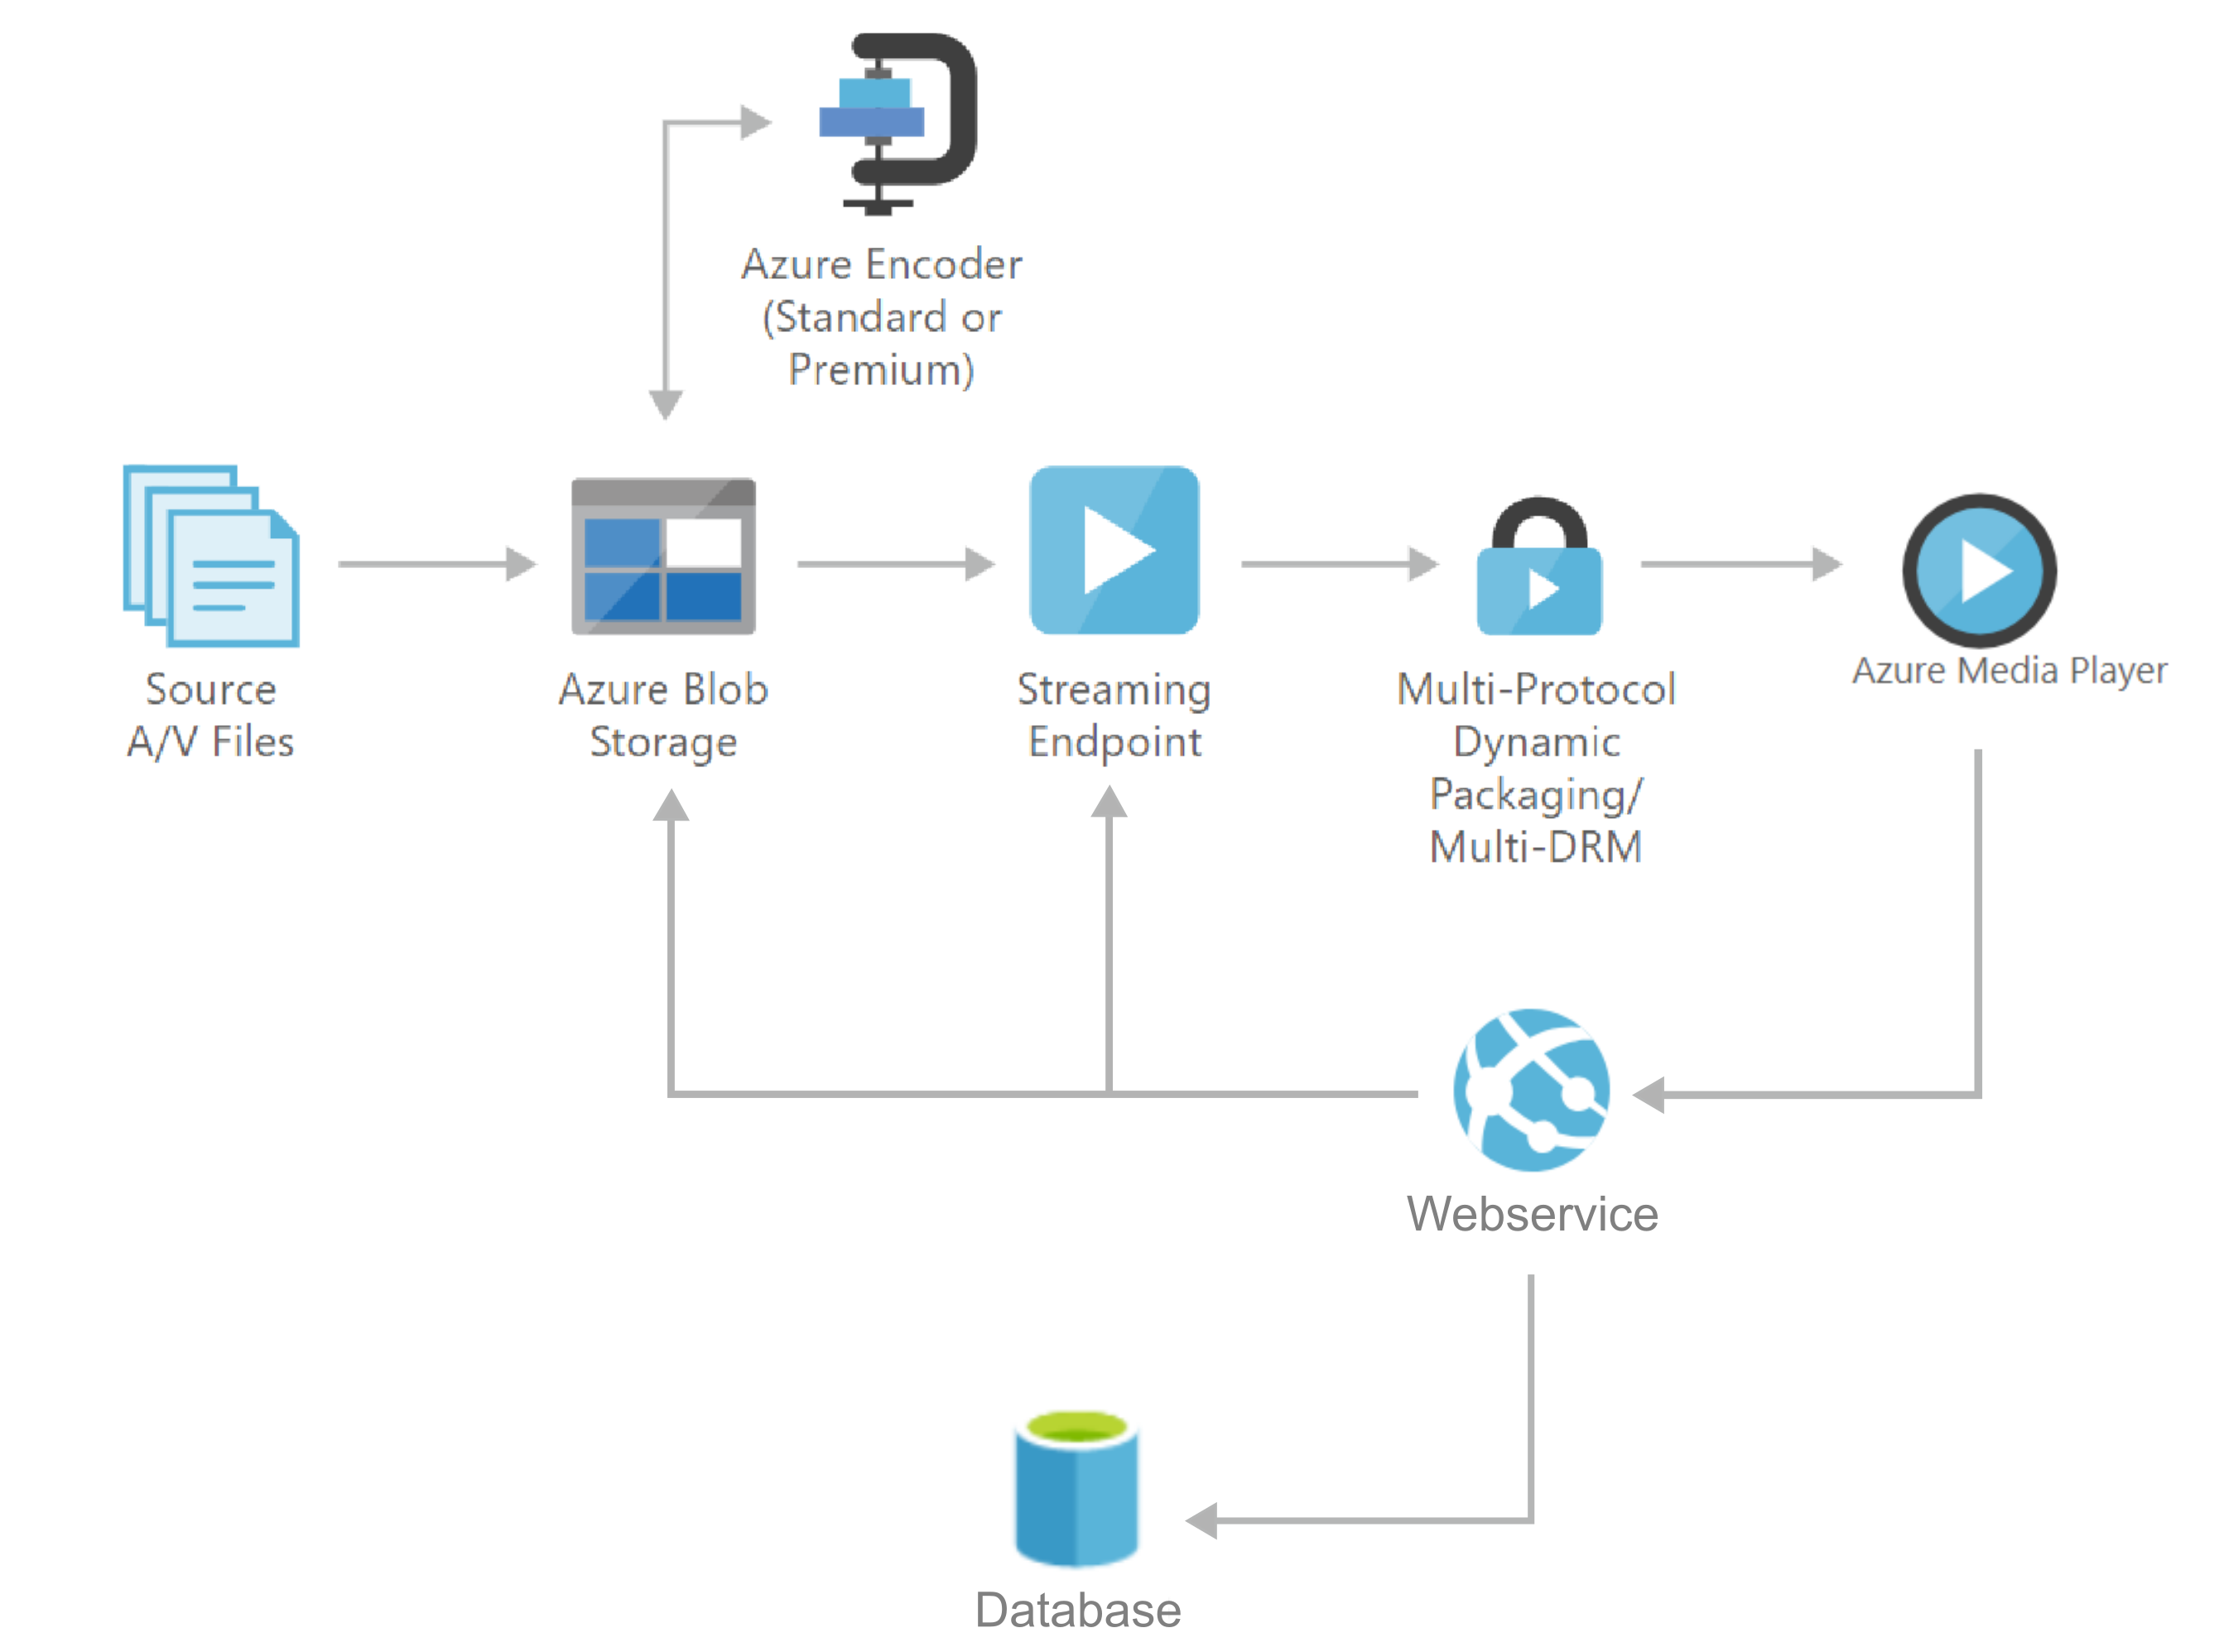
\includegraphics[width=1\textwidth, height=240px]{ressources/architecture_new.png}
    \caption{Modificated implementation of Microsofts VoD architecture}
    \label{fig:arch_new}
  \end{figure}
% ACuch benötigt laut config.js:  Azure ActiveDirectory (aad) id, secret, tenantID
% das hier?    https://docs.microsoft.com/de-de/azure/active-directory/develop/howto-create-service-principal-portal#create-an-azure-active-directory-application
% jap, steht in depl-script, auskommentiert. einmalige ausführung

Using Media Services results in a \textit{two-tier} server-architecture, in which the NodeJS-powered AppService has the end-user's devices as clients. The webserver itself is a client to the Azure Media Services Backend, requesting Encoding- and Streaming-Tasks by submitting \textit{Jobs}. This is also for security reasons, as Media Services uses a separate account-system with it's own credentials, generated by Microsoft. Those are confidential and must not be exposed to end-users. CORS (Cross Origin Resource Sharing) must be enabled for the Storage Account. 

The cloud components used scale completly automatic when needed. The NodeJS AppService is configurated to scale along the workload of the CPU resulting in creating another instance of the service. This happens once the defined threshold is reached. Incoming requests will automaticly distributed by Azure. The database behaves in the same way, scaling up and down when needed depending on the used price tier.
As defined by the US-based \textit{National Institute of Standards and Technology} (NIST) a cloud service must fulfill
certain criteria \cite{nistCloud}. This section gives a brief overview and reviews the application's fulfillment of each.
\begin{itemize}
    \item \textbf{On-Demand Self Service:} Users can create and scale resources through the aforementioned (ch2) user interfaces at any time and to any capacity they desire. Only starting up and allocating resources takes some time.
    \item \textbf{Broad Network Access:} Provided, as Microsoft holds a global server network and content can be delivered as HTML to be viewed in browsers on supporting devices.
    \item \textbf{Resource Pooling:} Resources can be organized in logical groups, but that's not the point. Resources of the provider are shared between multiple users, called 'tenants'.
    \item \textbf{Rapid Elasticity:} illusion of infinite resources \& scaling: provided by Azure as far as end users are concerned because everyone demands it. so MS has a trained 
    crew steadily working to administrate farms\\
    autoscaling however is only horizontally (more/less instances of the same resource). Vertical scaling (more powerful versions of instances) requires manual action, especially because the shift in price between tiers can be dramatic.
    \item \textbf{Measured Services:} provided by azure: Insights and Billing, Alerts
\end{itemize}

% Tabelle mit der Kostenaufstellung von Azure, skalierbare Elemente
% in versch. Tiern, also am Anfang nur 100GB BlobStorage, später 1TB, dann 10TB
% Kosten am Anfang (Tier 1): ca. 40 Euro im Monat, also mit einem Hartz4-Satz fast ein Jahr lang bezahlbar
% Das teuerste ist anfangs der AppService
% Finanzierung wird erst ein Problem, wenn viel mehr Content und Traffic anfallen
Using CDN is preferable, because ``When Azure CDN is not enabled for Media Services, data transfer is charged at Data Transfer Pricing. When Azure CDN is enabled for Streaming Units, data transfer charges do not apply. Data transferred is instead just charged at standard CDN pricing.'' 
% https://azure.microsoft.com/en-us/pricing/details/cdn/   vs   https://azure.microsoft.com/en-us/pricing/details/bandwidth/
While at first the pricing for both is near identical, it's the range from the 50th on to the 150th TB in one month that already shows the disparity: \$0.07 per GB through standard file transfer vs  \$0.0037 via CDN.
Bandwidth and CDN are also priced differently depending on region

According to an online filesize calculator \footnote{\url{https://toolstud.io/video/filesize.php}} a 25 FPS FullHD-Video of 20 minutes length would estimate to around 1 GB in size (average between \textit{YoutubeHD} and \textit{NetflixHD} with a necessary bandwidth of 8Mbps (1MB/s) in case of \textit{YoutubeHD} bitrate.  % ?imagewidth=1920&imageheight=1080&framerate=25&timeduration=60&timeunit=minutes
Assume that after a good start there are now 100 videos as the one described before. A total of 500 visitors arrive each month and watch 2 videos each: $(500 \ast 2 GB) = 1TB$ Streaming Throughput and $(500 \ast 2 \ast 20 min)  = 2000$ minutes (33,33 hours) of streamed video. (1000GB * 0,08ct) = 80 dolurs
The necessary blob storage amounts to $100 \ast 1GB = 100GB$. 
Let's also assume we receive 10 new videos each month, which results in an encoding output of $(10 \ast 20 mins) = 200$ minutes (6.75 dolurs).  

This brings us to a rough estimate (appsrv+streaming + encoding + storage) of 130 dolls each month. Spreading the costs to the users means every user uses services worth (130 / 500) = 0,26ct. If we omit the costs for the AppService and only account for costs generated through user interaction we get (90 / 500) = 0,18ct per user. The AppService is a mostly fixed cost as it is billed per running time, but media services costs scale upwards with user interaction.

Kosten: 80/20 Creator / SciTube
Every encoding costs: $Length * BasePriceHD$
Every view costs: $VideoSize * (Streaming+CDN)$
Every vid costs: $Size * StoragePrice$
Every month costs: $AppServiceBasePrice * Throughput$

\section{Conclusion and Future Work}\label{sec:ch6}
%CDN can be deployed and used easily but is not really needed right now. Scaling needs to be tested under real conditions (1000 -> 100000 Users), but only bc we need to know what to configure. Can assume that it works from a technical standpoint, as MS has way more experience
    % https://medium.com/@Traverous/the-tale-of-how-we-built-on-demand-streaming-for-traverous-on-azure-media-services-87e32f6a98d0
    %  https://devblogs.microsoft.com/premier-developer/how-to-setup-live-streaming-server-using-azure-media-service-in-less-than-30-mins/
    % https://docs.microsoft.com/de-de/azure/media-services/previous/media-services-streaming-endpoints-overview

As it turns out, setting up a globally scalable solution is relatively simple
using Microsoft's public cloud services. But consciously monitoring usage and resulting
expenses is critical as it's easy to accidentally choose an option that increases costs exponentially.
%In der Zukunft muss sich über ein Finanzierungsmodell gedanken gemacht werden. Ein möglicher Ansatz ist eine Mischung aus Werbefinanzierung und Abonement, ähnlich des Modells von Spotify. Eine Einteilung der Benutzer in Premium und Freemium ist von nöten. Freemium-User bekommen in regelmäßigen Abständen Werbung zu sehen, während Premium-User keine Werbung erhalten, aber monatlich einen finanziellen Beitrag bezahlen müssen.
%Ebenfalls muss die Verteilung des Inhalts von einem Storage über ein CDN-Netzwerk von statten gehen. Dies ermöglicht den weltweit schnellen Zugriff auf Inhalte ohne große Verzögerungen. 
In the future, a final financing plan must be implemented. Some attempts were 
already discussed in the previous chapter. Instead of using one plan straight, 
after acquiring users (financing by advertising), a subscription model could be 
implemented (free minutes at a discount if bought in advance).
Another possibility would be a \glqq rent-or-buy\grqq system similar
to Amazon Prime Instant Video. \\% in the true spirit of offering a 'service'
Also of interest is the Azure Media Clipper widget, which offers basic video cutting
functionality in a browser, allowing users to specifiy preview segments. AMS allows to
either encode such snippets as separate videos (adding further costs for encoding which
cannot be estimated) or to set \textit{filter rules} on existing media. Those should be
preferred as they are minimal in size and come at negligible further costs.\\
On the technical side, a CDN component should be implemented for a broad global 
reach and to minimize the costs as mentioned in chapter \ref{sec:ch5}. Also 
scaling needs to be tested under real conditions to find out the indicating 
parameter.
On one hand uploading the file from the user directly to the Azure Media Service 
would increase the performance of the application as well. On the other hand it 
would decrease the quality of service.\\
Lastly, the newly passed EU copyright directive opens up a completely new set of 
unanswered questions and problems for start-ups and content distributors in general.
Those problems can and should not be tackled without costly legal advice.


%  https://www.researchgate.net/profile/Chen_Wang30/publication/325922789_Comparing_Cloud_Content_Delivery_Networks_for_Adaptive_Video_Streaming/links/5b2c81564585150d23c1c024/Comparing-Cloud-Content-Delivery-Networks-for-Adaptive-Video-Streaming.pdf



\newpage
\appendix

%tables
\section*{Tables}
% https://www.tablesgenerator.com/latex_tables#
% https://de.overleaf.com/learn/latex/Tables
%
% Please add the following required packages to your document preamble:
% \usepackage[table,xcdraw]{xcolor}
% If you use beamer only pass "xcolor=table" option, i.e. \documentclass[xcolor=table]{beamer}

% \usepackage{lscape}  % rotation
        % \begin{landscape}
        % \end{landscape}
% \usepackage[normalem]{ulem}
% \useunder{\uline}{\ul}{}
\begin{landscape}
        \begin{table}[]
                \begin{tabularx}{\linewidth}{|l|X|X|X|}        % \begin{tabular}{c||c|c|c{10cm}|c}    geht auuuuuuuuuuuch nich, das formatieren soooo <.<
                \hline
                \multicolumn{3}{|l|}{{\ul \textbf{Microsoft Azure Estimate 1/2}}}                     & {\ul \textbf{SciTub Basic}}                         \\ \hline
                \textbf{Service type}             & \textbf{Custom name}      & \textbf{Description}                                                                                                                                                                                                                             & \textbf{Estimated Cost}                  \\ \hline\hline
                \textbf{Storage}                  & table storage 1gb         & Table Storage, Standard, LRS Redundancy, 1 GB Capacity, 100 Storage transactions                                                                                                                                                                 & \$0,11                                   \\ \hline
                \textbf{Azure Backup}             &                           & Azure VMs Type, 1 Instance(s) x 0 GB, LRS Redundancy, Moderate Average Daily Churn, 30 Daily RPs, 0 Weekly RPs, 0 Monthly RPs, 0 Yearly RPs,  After 1st year Duration, 0 Total Storage                                                           & \$0,00                                   \\ \hline
                \textbf{App Service}              &                           & Basic Tier; 1 B1 (1 Core(s), 1.75 GB RAM, 10 GB Storage) x 730 Hours; Linux OS                                                                                                                                                                   & \$38,69                                  \\ \hline
                \textbf{Content Delivery Network} &                           & Zone 1: 20 GB, Zone 2: 0 GB, Zone 3: 0 GB, Zone 4: 0 GB, Zone 5: 1 GB, DSA: 0 GB                                                                                                                                                                 & \$1,78                                   \\ \hline
                \textbf{Load Balancer}            &                           & Basic Load Balancer is free of charge                                                                                                                                                                                                            & \$0,00                                   \\ \hline
                \textbf{Application Gateway}      &                           & Basic tier, Medium Instance size: 0 Gateway hours instance(s) x 730 Hours, 0 TB Data processed unit(s), 5 GB Zone unit(s)                                                                                                                        & \$0,00                                   \\ \hline
                \textbf{IP Addresses}             &                           & 1 Dynamic IP Addresses, 5 Static IP Addresses, 0 Remaps                                                                                                                                                                                          & \$0,00                                   \\ \hline
                \end{tabularx}
                \caption{Azure Pricing Estimate Basic 1/2}
                \label{azPriceT1_1}
        \end{table}
\end{landscape}
\newpage
\begin{adjustbox}{angle=90}
    \begin{tabularx}{\textheight}{|l||X|m{4cm}|}        % \begin{tabular}{c||c|c|c{10cm}|c}    geht auuuuuuuuuuuch nich, das formatieren soooo <.<
    \hline
    \multicolumn{2}{|l|}{{\ul \textbf{Microsoft Azure Estimate 2/2}}}                     & {\ul \textbf{SciTub Basic}}                          \\ \hline \hline
    \textbf{Service type}            & \textbf{Description}                                                                                                                                                                                                                             & \textbf{Estimated Cost}                  \\ \hline\hline
    \textbf{Storage} (Temporary for uploading/encoding)                     & Block Blob Storage, General Purpose V1, LRS Redundancy, 10 GB Capacity, 100 Storage transactions                                                                                                                                                 & \$0,28                                   \\ \hline
\textbf{Storage} (Blob for Streaming)                           & Block Blob Storage, Blob Storage, LRS Redundancy, Hot Access Tier, 50 GB Capacity, 100,000 Write operations, 100,000 List and Create Container Operations, 100,000 Read operations, 100 Other operations. 10 GB Data Retrieval, 10 GB Data Write & \$2,08                                   \\ \hline
\textbf{Support}                                  & Basic Support                                                                                                                                                                                                                                          & \$0,00                                   \\ \hline
                                                        & Licensing Program                                                                                                                                                                                                                                & Microsoft Online Services Program (MOSP) \\ \hline
            \multicolumn{3}{|l|}{}                \\ \hline\hline
                                                       & \textbf{Monthly Total}                                                                                                                                                                                                                           & \textbf{\$42,93}                         \\ \hline
                                                       & \textbf{Annual Total}                                                                                                                                                                                                                            & \textbf{\$515,16}                        \\ \hline
\end{tabularx}
\label{tab:azPriceT1_2}
\end{adjustbox}
\newpage

%images
\section*{Images}
\begin{figure}[ht]
    \centering
    \includegraphics[width=1\textwidth, height=180px]{ressources/architecture_ms.png}
    \caption{Microsofts proposed VoD architecture}
    \label{fig:arch_ms}
\end{figure}
% plain bibtex:
%\bibliographystyle{lni}
%\bibliography{mybibfile}

%biber + biblatex
\printbibliography

\end{document}
